\section{Methodik}
\label{sec:methodik}

Zur erfolgreichen Durchführung umfassender Benchmarks setzen wir auf eine flexible Softwarearchitektur, welche eine einfache Parametrierung von vorhandenen MPI Schemata erlaubt. Diese Ansatz wird nachfolgend erläutert.

\subsection{Softwarearchitektur}
Die Softwarearchitektur des Projekts setzt auf zwei wesentlichen Prinzipien auf:
\begin{enumerate}
	\item Parameter structs für Value Iteration (TODO: abbreviation), MPI und Logging dienen als leichtgewichtige Umsetzung des Flyweight Patterns~\citep[S.195ff.]{gamma1995design}. Dieses Vorgehen erlaubt das unkomplizierte Lesen und Schreiben von Parametern, Laufzeitgrößen zur Steuerung und Messwerten ohne Kopien.
	\item Eine an MVC~\citep[S.125ff.]{buschmann1996pattern-oriented} angelehnte und durch das Flyweight vernetzte Struktur. Diese besteht aus generischer Value Iteration (TODO: abbreviation) Implementierung (Model), flexibler Eingabe von Steuergrößen und Ausgabe von Messwerten (View) und verschiedenen, interfacekompatiblen MPI Schemata (Controller).
\end{enumerate}

\subsection{Automatisierung}
Aufbauend auf der flexiblen Softwarearchitektur konnten wir eine weitgehende Automatisierung der Messdatenerfassung und -auswertung erzielen. Wie das Ablaufdiagramm (TODO: add ref) zeigt, bietet das Projekt verschiedene make Targets für die jeweiligen Ausführungsumgebungen. Diese werden in \ref{ssec:ausfuehrungsumgebungen} genauer aufgeführt. Jedem dieser Testziele ist gemein, dass die Ausführung vollständig automatisiert auf Basis eines mehrstufigen Konfigurationsprozesses abläuft. In der ersten Stufe können die gewünschten Messzyklen und zu testenden Processorcounts je Datensatz vorgegeben werden. Diese werden schließlich auf jeder der Konfiguration angewandt, welche mittels eines Testauftraggenerators erzeugt werden. Dieser kann mittels YAML-Dateien (TODO: Referenz) konfiguriert werden und erlaubt es, die zu testenden Kombinationen aus Datensatz, MPI Kommunikationsintervall und MPI Schema zu definieren. Der Generator speichert hierzu je Auftrag eine YAML-Datei ab, welche sich über einen Vererbungsprozess einer definierten Standardkonfiguration des Testziels bedient.

Der eigentliche Test iteriert nun entsprechend der gewählten Anzahl Zyklen und Varianten Processorcount über die Testaufträge und arbeitet je einen Auftrag mittels eines Aufrufs von mpirun ab. Jeder dieser Durchläufe schreibt eine Reihe von Mess- und Kenngrößen in eine CSV-Datei in ein automatisch erzeugtes Verzeichnis. Dieses Verzeichnis wird automatisiert vor und nach einem Test mittels rsync auf eine HiDrive Instanz von Strato synchronisiert, sodass jeder Tester zu jeder Zeit alle aktuellen Messdaten zur Verfügung hat.
Um eine hohe Reproduzierbarkeit zu gewährleisten, werden die Testdatei zudem mittels Metainformationen wie aktiviertem git Branch, git Commit Hash (mit dirty Erkennung), genutzter Testumgebung und git User-Email des Testers abgespeichert. Hiermit lässt sich stets auf den genutzten Softwarestand schließen, welcher den erzeugten Messdaten zugrundeliegt.

Eine Erkenntnis aus der Anwendung dieses Systems auf die HPC Cluster der TUM ist die Relevanz der Testausführung: werden Zyklen gleicher Testaufträge hintereinander abgearbeitet ergibt sich eine hohe Vergleichbarkeit der Daten durch gleiche Rahmenbedingungen. Liegen hierbei anhalten schwierige Bedingungen, z.B. durch eine hohe Auslastung durch andere Nutzer, vor, führt dies jedoch zu suboptimalen Messdaten für alle Zyklen. Die vorliegenden Daten sind zur Besserung Interpretierbarkeit daher mit der ersten Variante erzeugt worden.

\subsection{Ausführungsumgebungen für Tests}
\label{ssec:ausfuehrungsumgebungen}
Um plattformspezifische Einflüsse wie Betriebssystem, Hardware oder Netzwerktechnik vermeiden zu können, haben wir die Automatisierung auf eine Reihe von Testumgebungen angewandt. Die Daten von sechs dieser Umgebungen bilden die Grundlage für unsere Analysen und werden zusätzlich in Bezug mit der dieser Ausarbeitung zugrundeliegenden Implementierung der asynchronen Value Iteration mittels OpenMP verglichen. Die Testumgebungen sind folgende:

\begin{enumerate}
	\item HPC Class A: Bis zu 5 (hpc01 - hpc05) PCs des LDV mit je einer Vierkern-CPU und 8GB RAM
	\item HPC Class B: Bis zu 10 (hpc06 - hpc015) PCs des LDV mit je einer Vierkern-CPU und 8GB RAM
	\item HPC Class Mixed: Bis zu 15 (hpc01 - hpc015) PCs des LDV mit je einer Vierkern-CPU und 8GB RAM
	\item HPC NUC: 2 NUC Computer mit je einer Zweikern-CPU und 32GB RAM
	\item HPC RPi: 4 RaspberryPi Single-Board-Computer mit je einer Vierkern-CPU und 8GB RAM
	\item Lokal: 1 PC (hpc04) des LDV mit einer Vierkern-CPU und 8GB RAM
\end{enumerate}

In Summe liegen dieser Ausarbeitung schließlich Messdaten entsprechend \autoref{fig:NumberMeasurementsSmall} und \autoref{fig:durationMeasurementsSmall} für den Datensatz <small> und \autoref{fig:NumberMeasurementsNormal} und \autoref{fig:durationMeasurementsNormal} für den Datensatz <normal> zugrunde.

\begin{figure}[h]
	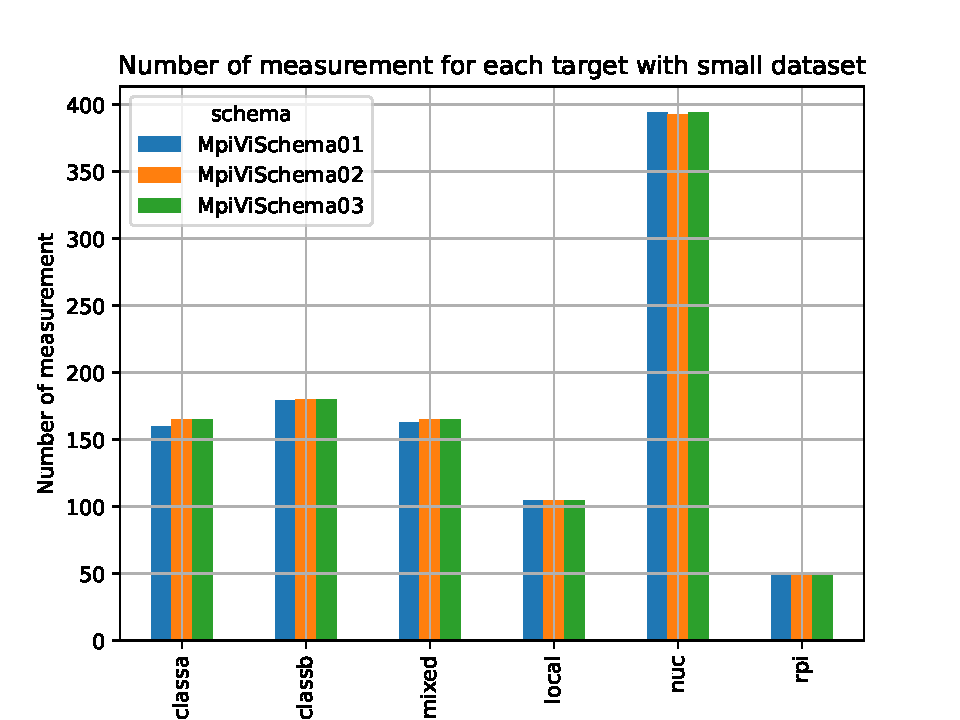
\includegraphics[width=0.5\textwidth]{./gen/img/ds/small/number_measurement_target.pdf}
	\caption{Anzahl an Messungen pro Rechenklasse mit kleinem Datensatz}
	\label{fig:NumberMeasurementsSmall}
\end{figure}

\begin{figure}[h]
	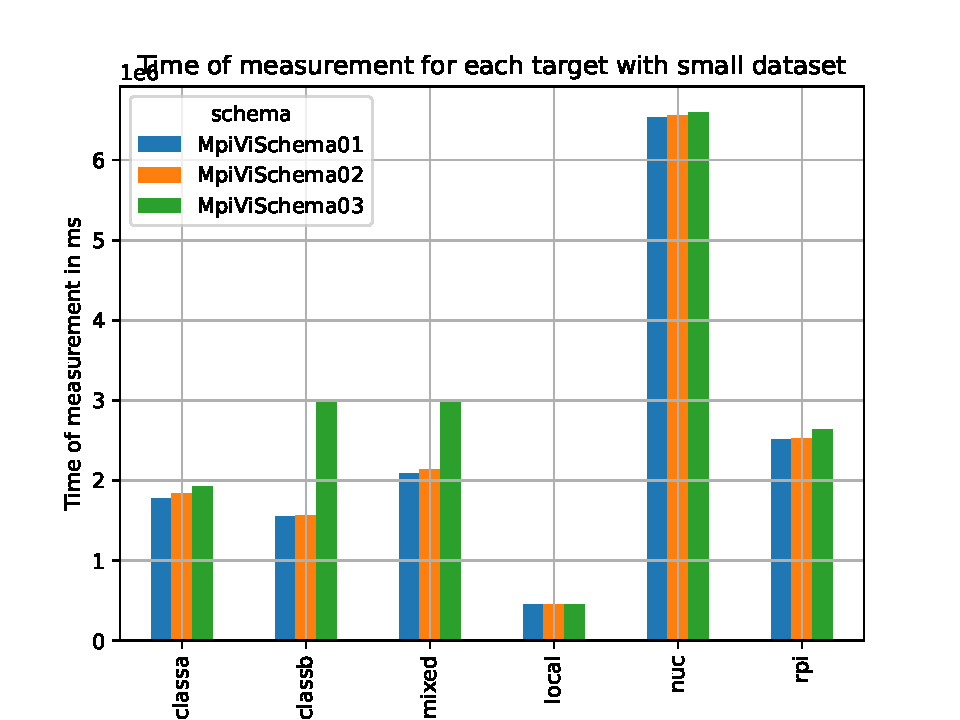
\includegraphics[width=0.5\textwidth]{./gen/img/ds/small/runtime_measurement_target.pdf}
	\caption{Gesamtdauer an Messungen pro Rechenklasse mit kleinem Datensatz}
	\label{fig:durationMeasurementsSmall}
\end{figure}

\begin{figure}[h]
	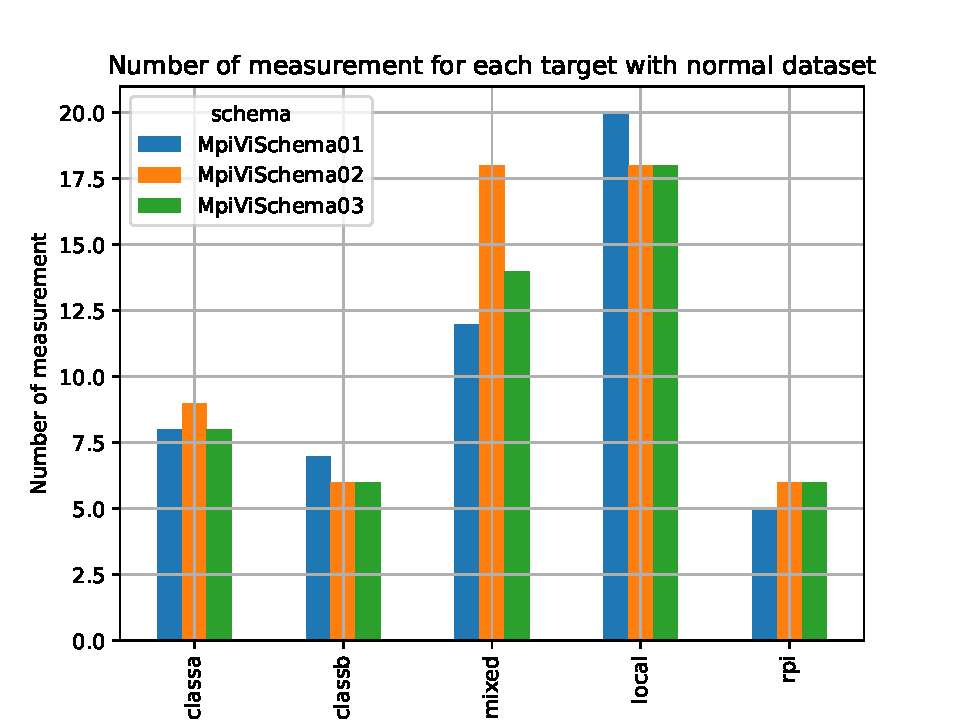
\includegraphics[width=0.5\textwidth]{../gen/img/ds/normal/number_measurement_target.pdf}
	\caption{Anzahl an Messungen pro Rechenklasse mit normalen Datensatz}
	\label{fig:NumberMeasurementsNormal}
\end{figure}


\begin{figure}[h]
	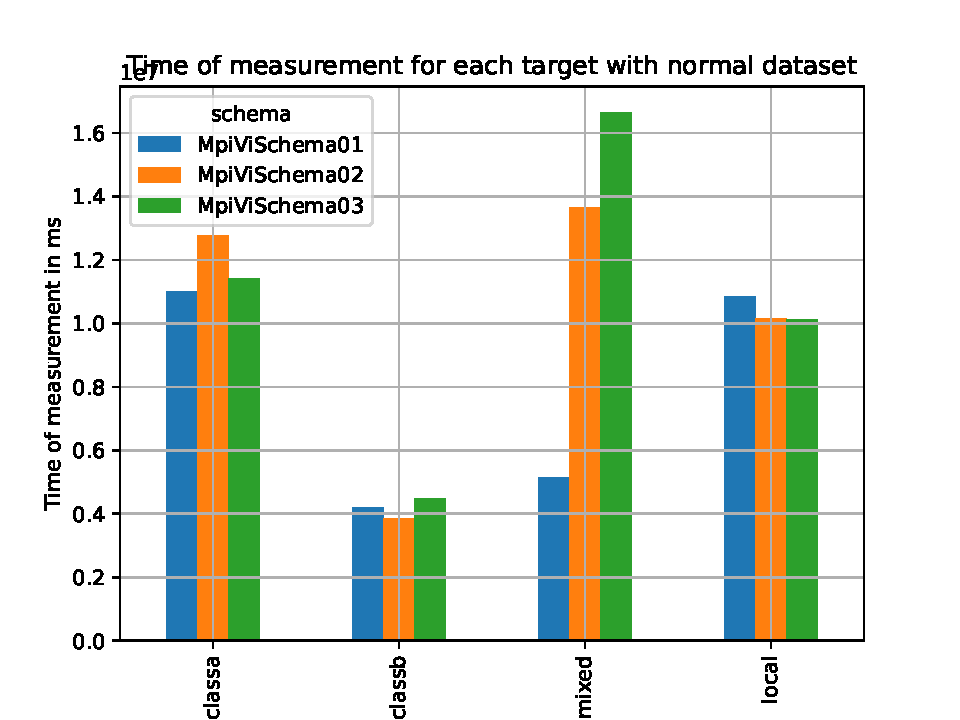
\includegraphics[width=0.5\textwidth]{../gen/img/ds/normal/runtime_measurement_target.pdf}
	\caption{Gesamtdauer der Messungen pro Rechenklasse mit normalen Datensatz}
	\label{fig:durationMeasurementsNormal}
\end{figure}

\subsection{Schemata}
\label{ssec:schemata}

Den Kern dieser Arbeit bildet die Validierung und das Benchmarking verschiedener Kommunikationsschemata mittels Open MPI. Hierzu wurden drei Schemata implementiert, welche nachfolgend vorgestellt werden sollten. Außerhalb der eigentlichen Schemata ist eine Verteilung der Testkonfiguration und Aggregation von Messgrößen von/zu dem Processor mit Rank0 mittels verschiedener MPI Mechanismen realisiert.

\subsubsection{MpiViSchema01}
Das erste Schema \autoref{fig:mpiViSchema01} ist ein synchronisiertes Schema, welches einen Zugriff auf den Datensatz bei jedem Processor voraussetzt. Dieses Schema nutzt die MPI Mechanismen Allgatherv zur Synchronisation des aktuellen Kostenvektors, Allreduce zur Bestimmung eines globalen Konvergenzkriteriums eps und Gatherv zur Bereitstellung des globalen Aktionsvektors.

\begin{figure}[h]
	\centering
	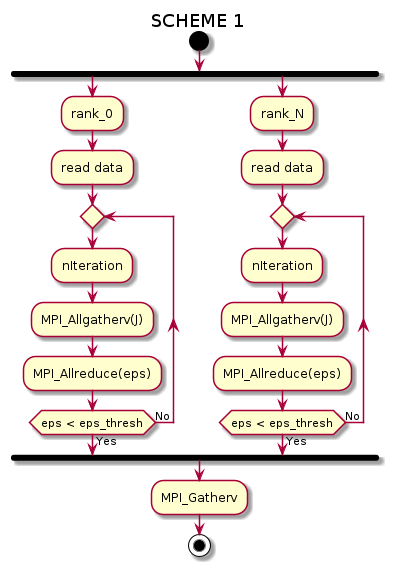
\includegraphics[width=0.3\textwidth]{/home/tobias/git/ldv/gruppe-3-hauptprojekt-doc/rep/gen/puml/scheme1}
	\caption{MpiViSchema01}
	\label{fig:mpiViSchema01}
\end{figure}

\subsubsection{MpiViSchema02}
Das Schema Nummer zwei \autoref{fig:mpiViSchema02} ist ebenfalls ein synchronisiertes Schema, welches jedoch als wesentlichen Unterschied eine Verteilung des Datensatzes ausgehend vom Processor mit Rank0 umsetzt. Hierbei müssen andere Processors mitunter keinen Zugriff auf die Datensätze haben und können somit mit weniger Arbeits- und Festspeicher arbeiten. Dieser Vorgang wird mittels des MPI Mechanismus Scatterv umgesetzt und implementiert eine aufwändige Spaltung des Datensatz in abgeschlossene Blöcke, wovon jedem Processor nur einer vorliegt. Die eigentliche Ablauf der Value Iteration erfolgt vergleichbar zu Schema01.

\begin{figure}[h]
	\centering
	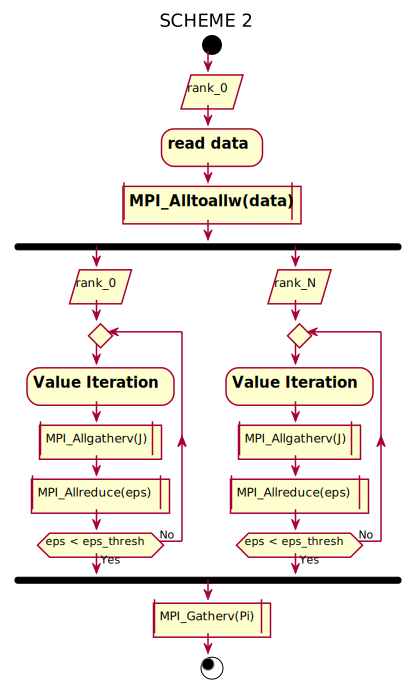
\includegraphics[width=0.3\textwidth]{/home/tobias/git/ldv/gruppe-3-hauptprojekt-doc/rep/gen/puml/scheme2}
	\caption{MpiViSchema02}
	\label{fig:mpiViSchema02}
\end{figure}

\subsubsection{MpiViSchema03}
Das dritte und letzte Schema \autoref{fig:mpiViSchema03} dieser Ausarbeitung ist ebenso ein synchrones Schema, nutzt statt optimierter Routinen für den großflächige Datenaustausch jedoch die trivialen MPI Methoden wie Sendv und Recv zum Austausch des Kostenvektors J und des Konvergenzkriteriums eps.

\begin{figure}[h]
	\centering
	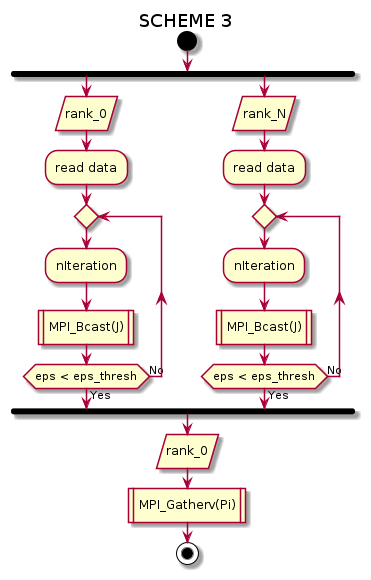
\includegraphics[width=0.3\textwidth]{/home/tobias/git/ldv/gruppe-3-hauptprojekt-doc/rep/gen/puml/scheme3}
	\caption{MpiViSchema03}
	\label{fig:mpiViSchema03}
\end{figure}

\section{Analyse \& Diskussion}
\label{sec:analyse_diskussion}
Ziel dieses Kapitels ist es Parameter die Einfluss auf die Berechnung nehmen hervorzuheben und die drei oben erw\"ahnten implementierten Schemen zu analysieren. Dabei soll der Fokus vorallem auf der Rechenzeit, den Speicherbedarfs und den Rechenfehler liegen. \\ Um die  Schemta zu Vergleichen wurden Testl\"aufe mit unterschiedlichen Parametern gemessen. Diese Ergebnisse werden in Unterkapitel A er\"ortert. Um erworbene Erkenntnisse auf anderen Systemen zu verifizieren wurden Messungen auf verschiedenen Klassen an Recheneinheiten ausgef\"uhrt. Dies wird in Unterkapitel B beschrieben. Zu den verwendeten Klassen geh\"oren: HPC Klasse A (HPC 1 - HPC 5), HPC Klasse B (HPC 6 - HPC 15), eine gemischte HPC Klasse (HPC 1 - HPC15) und aus privat stammendem Besitz  Raspberry Pi Klasse, NUC Rechnerklasse und eine lokale Rechnerklasse. \\ Da es teilweise auf den Messger\"aten zu einer ungleichm\"a\ss{}igen Auslastung kam und damit Datenausrei\ss{}er generiert wurden, wurden pro Messzyklen mehrere Messungen durchgef\"uhrt. Die Anzahl und Messzeiten pro Ger\"at und Schema k\"onnen der Abbildung (\ref{fig:NumberMeasurementsSmall} und \ref{fig:NumberMeasurementsNormal}) entnommen werden. Auf allen Messger\"aten wurden Messungen mit je dem klein und normal gro\ss{}en Datensatz vorgenommen. Die in diesem Kapitel angesprochenen Grafiken und weitere Grafiken sind der \"Ubersicht halber im Anhang abgebildet.

\subsection{Vergleich der Schemata}
Bei den Messdaten die \"uber die Anzahl an Recheneinheiten und dem Kommunikationsintervall variieren, kann gesehen werden, dass es zwischen den einzelnen Schemen, in Bezug auf Rechenzeit und Konvergenzschritten, zu keinen gro\ss{}en Unterschieden kommt. Dies kann den Messungen auf den Nuc Rechnern aus der Grafik (\ref{fig:NUCworldTimesmall}) und der Grafik (\ref{fig:NUCStepWorldSizesmall}) besonders gut entnommen werden. Dennoch k\"onnen mit steigender Anzahl der Recheneinheiten  etwas schnellere Ergebenisse erziehlt werden, siehe Grafik (\ref{fig:hpcBworldTimesmall}). Allerdings kann der Gewinn an Rechenzeit durch die Parallelisierung von Rechenschritten bei einer zu gro\ss{}en Anzahl an Recheneinheiten, durch den den gro\ss{}en Kommunikationsaufwand, schnell wieder zunichte gemacht werden, wie in Abbilung (\ref{fig:hpcMixedworldTimesmall}) gesehen werden kann. Die Anzahl der Recheneinheiten hat au\ss{}erdem eine Auswirkung auf die Anzahl der Iterationsschritte. So steigt mit der Anzahl der Recheneinheiten auch die Anzahl der ben\"otigten Iterationsschritte. Einen gro\ss{}en Einfluss auf die Rechenzeit hat das Kommunikationsintervall, siehe  Grafik (\ref{fig:NUCcomTimesmall}). So kann beobachtet werden, dass ganz am Anfang die Rechenzeit mit zunehmendem Kommunikationsintervall verk\"urzt werden kann. Doch tritt schon fr\"uh nach einer weitere Erh\"ohung des Kommunikationsintervalls eine Zunahme der Rechenzeit ein. Im von uns gew\"ahlten Kommunikationsintervall ist gegen Ende hin eine lineare Zunahme der Rechenzeit zu sehen, Grafik (\ref{fig:hpcMixedcomTimesmall}). Diese Zunahme der Rechenzeit resultiert vor allem aus einer h\"oheren Anzahl an ben\"otigten Iterationsschritten bis zur Konvergenz, siehe Grafik (\ref{fig:NUCIterationWorldSizesmall}). Es wird au\ss{}erdem aus der Grafik (\ref{fig:NUCIterationWorldSizesmall}) sichtbar, dass mit einem h\"oherem Kommunikationsintervall eine h\"ohere Varianz bei den Iterationsschritten entsteht. Diese entstehende Varianz ist bei allen gemessenen Schemen gleich ausgepr\"agt.\\ Auch bei der Frage des Speicherbedarfs k\"onnen einige Erkenntnisse gewonnen werden. Generell ist zu sehen, dass Schema 1 und Schema 3 beim Speicherbedarf nahe beieinander liegen. Schema 2 ben\"otigt auf der Recheneinheit mit dem Rang 0 einen deutlich h\"oheren Speicherbedarf als die anderen beiden Schemata. Wenn man jedoch den gesamten Speicher f\"ur die Recheneinheiten \"uber die Anzahl von Recheneinheiten anschaut, wie in Grafik (\ref{fig:LocalsumRSSsmall}), so sieht man dass mit h\"oherer Anzahl an Recheneinheiten der Speicherbedarf steigt. Bei Schema 2 jedoch nicht so stark wie bei den anderen Schemata. Daher ist etwa ab 4 Recheneinheiten besser das speicherärmere Schema 2 zu verwenden. Das k\"onnte mit dem Schemaaufbau erkl\"art werden, da hier nur ein Rang alle Daten einliest und erst danach auf die anderen Rechner weiterveteilt.\\
Bei der Analyse des Rechenfehlers ist es schwieriger anhand der gewonnenen Messdaten eine Aussage zu treffen, da die Messergebnisse je nach Rechnerklasse variieren k\"onnen.  Jedoch l\"asst sich sagen, dass der Mittelwert bei gleicher Parameterwahl und gleicher Rechnerklasse zwischen den Schemen wenig variiert. Dies gilt sowohl f\"ur die l2, die Maxnorm und die mittlere quadratische Abweichung. Au\ss{}erdem bleibt der Fehler je nach Recheneinheit mit varrierender Rechenanzahl und Kommunikationsintervall gleich, siehe Grafik (\ref{fig:NucWsJdiffssmall}) oder Grafik (\ref{fig:NuccomJdiffssmall}).\\

\subsection{Vergleich der Ausführungsumgebungen}
Beim Vergleich der verschiedenen Ausf\"uhrungsrechenklassen f\"allt vorallem auf, dass die Rechenzeit auf den Nuc, Lokalen und Raspberry PI Rechnern zwischen den implementierten Schemen weniger variiert. Da die Auslastung auf den HPC Rechnern, je nach Anzahl der Benutzer stark variiert, wird hier auch eine Varianz in den Rechenzeiten sichtbar. Da die Rechnergruppen jedoch unterschiedliche Rechenleistungen aufweisen, kann man keinen direkten Vergleich der Rechenzeit vornehmen. Dennoch k\"onnen bei der Analyse der Rechenzeit auf den verschiedenen Messger\"atklassen, Eigenschaften der verschiedenen Schemata aufgezeigt werden. So sieht man dass der Mittelwert der Rechenzeit bei gr\"o\ss{}eren Kommunikationsintervallen in der Mixed Klasse gr\"o\ss{}er ist als in Klasse B. Die Mixed Rechnerklasse HPC Rechner beinhaltet Rechner aus Klasse A und Klasse B. Dabei weist die Rechnerklasse A eine leicht schlechtere Rechenleistung auf, wie der Vergleich der mittleren Laufzeiten von Klasse A und Klasse B sich zeigt. Da nun in den implementierten Schemen bei der Kommunikation auf das langsamste Glied gewartet werden muss, kann die leicht homogen perfomantere Rechnerklasse schneller zu einem Ergebniss kommen.\\
Auch bei der Betrachtung des Rechenfehlers gab es Unterschiede zwischen den Rechnerklassen. So die wird Berechnungen auf Rechnerklasse A mit einem gr\"o\ss{}er Fehler ausgef\"uhrt als auf Rechnerklasse B. \\
Beim Vergleich der unterschiedlichen Ausf\"uhrungsergebnissen konnte jedoch meistens die Erkenntnisse aus dem Unterkapitel A auf allen Rechnerklassen best\"atigt werden. 

\section{Thesen}
\label{sec:thesen}

Der folgende Abschnitt behandelt Thesen bezüglich der Zusammenhänge zwischen Messgrößen und Parametern.
Die Thesen werden anhand der Messergebnisse, der zugrunde liegenden Schema-Architektur und Hardware erörtert.

\subsection{Es besteht eine Korrelation von RAM mit world\_size}

Wie zu erwarten steigt der summierte RAM-Bedarf über alle Processors mit steigender world\_size
(Fig \ref{fig:rssSumSmall} und Fig \ref{fig:rssSumNormal} sowie Fig \ref{fig:hpcAsumRSSsmall}-l, Fig \ref{fig:NUCsumRSSsmall}-l, Fig \ref{fig:hpcAsumRSSnormal}-l und Fig \ref{fig:NUCsumRSSnormal}-l).
Insbesondere bei Schema 1 und 3 liegt jedem Processor
die gesamte Datenmenge an Parametern und P-Matrix im Arbeitsspeicher vor.
Schema 2 teilt im Gegensatz dazu die P-Matrix in Blöcke auf und scattert diese an alle Processors.
Diese Aufteilung und dadurch, dass rank\_0 auch an sich selbst
scattert führt dazu, dass rank\_0 von Schema 2 einen höheren RAM Bedarf hat als bei Schema 1 und 3.
Weiterhin kann den Messungen entnommen werden,
dass ab einer world\_size von 4 beim kleinen Datensatz und 16 beim normalen Datensatz
der gesamt benötigte RAM Bedarf von Schema 2 niedriger als bei den anderen beiden Schemas ist und darüber
hinaus langsamer ansteigt.
Das liegt daran, dass jeder rank nur einen Bruchteil entsprechend der world\_size der Daten erhält und somit jede Vergrößerung der
world\_size einen niedrigeren durchschnittlichen RAM Bedarf ergibt.
In Fig \ref{fig:rssMaxSmall} und Fig \ref{fig:rssMaxNormal} sowie Fig \ref{fig:hpcAmaxRSSsmall}-l, Fig \ref{fig:NUCmaxRSSsmall}-l, Fig \ref{fig:hpcAmaxRSSnormal}-l und Fig \ref{fig:NUCmaxRSSnormal}-l
ist der maximal benötigte RAM-Bedarf von rank\_0 in jedem Schema dargestellt.
Der Bedarf bleibt über alle world\_sizes konstant, da jeder rank\_0
unabhängig von Schema und world\_size die gesamte Datenmenge im Arbeitsspeicher vorliegen hat.

\begin{figure}[h]
	\subfloat[max RSS, small]{
			\centering
			\includegraphics[width=0.25\textwidth]{./gen/img/ds/small/max_rss_rank0_world_size.pdf}
			\label{fig:rssMaxSmall}
    \hspace{0pt}}
	\subfloat[sum RSS, small]{
			\centering
			\includegraphics[width=0.25\textwidth]{./gen/img/ds/small/rss_sum_all_world_size.pdf}
            \label{fig:rssSumSmall}
	}\\
	\subfloat[max RSS, normal]{
       	\centering
    	\includegraphics[width=0.25\textwidth]{./gen/img/ds/normal/max_rss_rank0_world_size.pdf}
    	\label{fig:rssMaxNormal}
    \hspace{0pt}}
    \subfloat[sum RSS, normal]{
    	\centering
    	\includegraphics[width=0.25\textwidth]{./gen/img/ds/normal/rss_sum_all_world_size.pdf}
        \label{fig:rssSumNormal}
    }
	\caption{Verlauf des RSS-Bedarfs}
	\label{fig:NumberMeasurements}
\end{figure}

\subsection{Es besteht eine Korrelation runtime mit com\_interval}

Das com\_interval ist der Parameter, der angibt wie oft Ranks miteinander kommunizieren.
Anhand der Diagramme Fig \ref{fig:hpcAcomTimesmall}-f, Fig \ref{fig:NUCcomTimesmall}-f, Fig \ref{fig:hpcAcomTimenormal}-f
und Fig \ref{fig:NUCcomTimenormal}-f
ist eine klare Korrelation zwischen der benötigten runtime zur Konvergenz und com\_interval erkennbar. Zur Darstellung eines
eindeutigeren Verlaufs sind Messungen mit einer höheren com\_interval-Auflösung in Fig \ref{fig:ScatRunCom} und \ref{fig:ScatStepCom}
dargestellt. Die runtime ist bei allen drei Schemas sehr ähnlich und die Iterationsanzahl sogar meist identisch,
daher überdecken die Messpunkte von Schema 3 zum Großteil die anderen beiden Schemata. Die beiden nebeneinander verlaufenden Kurven resultieren
aus den zwei unterschiedlichen world\_sizes 2 \& 4. In Fig \ref{fig:ScatRunCom} gehört die Kurve mit niedrigerer runtime zu world\_size 4 und
in Fig \ref{fig:ScatStepCom} gehört der Verlauf mit höherer benötigter Iterationsanzahl zu world\_size 4.
Eine durch höheres com\_interval geringere Häufigkeit der Kommunikation zwischen den Processors führt dazu, dass die Processors
mehr Iterationen der Value Iteration durchführen bevor die Ergebnisse untereinander ausgetauscht werden.
Im Idealfall würde durch selteneres Austauschen weniger Zeit für eben diese Kommunikation verwandt werden und die runtime dadurch sinken.
Tatsächlich führt ein größeres com\_interval dazu, dass durch das seltenere
Update des J-Vektors die Konvergenz beinträchtigt wird. Das führt zu einer höheren benötigten Iterationsanzahl was schlussendlich
wieder zu einer höheren Anzahl an benötigten Kommunikationen und dadurch
zu einer längeren Laufzeit führt. Der ansteigende Bedarf an Iterationen bei steigendem com\_interval ist in Fig \ref{fig:ScatStepCom}
dargestellt.
Für die dargestellten NUC-Messungen haben diese beiden sich gegensätzlichen Effekte in Summe bei com\_interval 3 ihr Minimum.
Bei den anderen Targets liegt das Minimum ebenfalls in dieser Größenordnung. Ohne explizite Messung mit com\_interval 3 kann jedoch
kein Schluss daraus gezogen werden ob das Minimum bei com\_interval 3 hardware-unabhängig ist.

\begin{figure}[h]
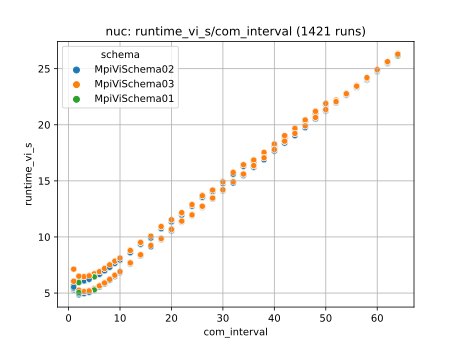
\includegraphics[width=0.5\textwidth]{./gen/img/nuc/small/scatterplot_com_interval_runtime_vi_s.pdf}
\vspace*{-8mm}
\caption{NUC, runtime\_vi vs. com\_interval, world\_size 2 \& 4}
\label{fig:ScatRunCom}
\end{figure}

\begin{figure}[h]
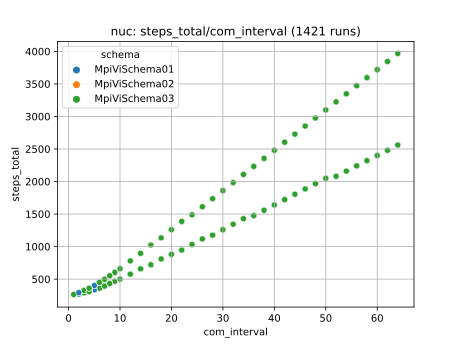
\includegraphics[width=0.5\textwidth]{./gen/img/nuc/small/scatterplot_com_interval_steps_total.pdf}
\vspace*{-8mm}
\caption{NUC, steps vs. com\_interval, world\_size 2 \& 4}
\label{fig:ScatStepCom}
\end{figure}

\subsection{Es besteht keine Korrelation zwischen world\_size und runtime}

Eine größere world\_size erhöht die Anzahl an Berechnungen, die parallel durchgeführt werden können.
Sind die Berechnungen pro Processor komplex/lange genug um den Mehraufwand an inter-Processor Kommunikation zu
rechtfertigen so führt dies zu einer veringerten runtime.
In der vorliegenden Value-Iteration ist der Effekt nicht besonders stark, da die Berechnungen für die nötige
Konvergenz nicht unabhängig voneinander durchgeführt werden können. Ein regelmäßiger Austausch der Ergebnisse während des Algorithmus ist für ein
richtiges Ergebnis zwingend nötig. Das führt zu einer notwendigen Kommunikation zwischen den Processors,
die dem Effekt der Zeitersparnis durch Parallelisierung entgegenwirkt.
Anhand der Messergebnisse in Fig \ref{fig:hpcAworldTimenormal}-c und Fig \ref{fig:NUCworldTimenormal}-c kann besonders beim normalen Datensatz
kein Zusammenhang zwischen der world\_size und der runtime festgestellt werden, da
die Auswirkung einer größeren world\_size von Target zu Target unterschiedlich ausfällt.
Bei den isolierten Targets NUC, RPi und Local bleibt die Zeit weitgehend gleich mit einer Tendenz zu geringfügig schnellerer Ausführung
bei größerer world\_size. Aufgrund der Varianz der Messdaten ist es jedoch nicht möglich eine zuverlässige Aussage darüber zu treffen.
Beim kleinen Datensatz (siehe Fig \ref{fig:hpcAworldTimesmall}-c und Fig \ref{fig:NUCworldTimesmall}-c) ist im Allgemeinen,
bis auf world\_size 56 bei HPC Class mixed, eine leichte Tendenz zur schnelleren Ausführung bei größerer world\_size zu beobachten.
Das liegt vermutlich daran, dass die HPCs frei zugänglich sind und die Wahrscheinlichkeit weiterer Nutzer, die die runtime
stören, mit steigender world\_size und grundsätzlich längerer Berechnungsdauer beim größeren Datensatz steigt.
Weiterhin sind die Schemata mit blockierenden MPI-Funktionen implementiert. Das bedeutet, dass in jeder Kommunikations-Iteration
auf den langsamsten Processor gewartet wird. So führt die Heterogenität beim mixed-cluster zu Performance Einbußen, weiterhin
müssen alle genutzten Processors warten, falls ein Processor durch einen zusätzlichen Nutzer am HPC verlangsamt wird.
Für eine eindeutige Aussage der genauen Korrelationen sind Messungen mit garantiert freiem Cluster und kontrollierten Störungen nötig.
Im Vergleich zur asynchronen Value Iteration ohne MPI-Kommunikation (siehe Tabelle \ref{tab:vergleich}) zeigt sich, dass im vorliegenden Fall der Value Iteration beim großen Datensatz die Nutzung von MPI zu keiner Verbesserung der
Performance führt.
Beim kleinen Datensatz konnte bei HPC class A mit world\_size 12 und HPC class B mit world\_size 30 der openMP-Wert unterschritten werden.
Allerdings ist die Varianz der Zeiten so hoch, dass im Mittel kein Performance Gewinn erreicht wird.

\begin{table}[h]
\caption{Vergleich der runtime von openMP und MPI}
\resizebox{\linewidth}{!}{
\begin{tabular}{l|c|c|c|c}
 Datensatz &\multicolumn{2}{c|}{HPC class A} & \multicolumn{2}{c}{HPC class B}\\
 \hline
 & openMP & MPI & openMP & MPI\\
 \hline\hline
small & \textasciitilde 5s & \textasciitilde 4-11s & \textasciitilde 3.5s & \textasciitilde 2-10s \\
normal & \textasciitilde 490s & \textasciitilde 600-800s & \textasciitilde 360s & \textasciitilde 400-600s \\
\label{tab:vergleich}
\end{tabular}}
\end{table}